\documentclass[11pt]{article}
\usepackage[scaled=0.92]{helvet}
\usepackage{geometry}
\geometry{letterpaper,tmargin=1in,bmargin=1in,lmargin=1in,rmargin=1in}
\usepackage[parfill]{parskip} % Activate to begin paragraphs with an empty line rather than an indent %\usepackage{graphicx}
\usepackage{amsmath,amssymb, mathrsfs, dsfont}
\usepackage{tabularx}
\usepackage[font=footnotesize,labelfont=bf]{caption}
\usepackage{graphicx}
\usepackage{xcolor}
%\usepackage[linkbordercolor ={1 1 1} ]{hyperref}
%\usepackage[sf]{titlesec}
\usepackage{natbib}
\usepackage{../../Tianpei_Report}
%\usepackage{appendix}
%\usepackage{algorithm}
%\usepackage{algorithmic}

%\renewcommand{\algorithmicrequire}{\textbf{Input:}}
%\renewcommand{\algorithmicensure}{\textbf{Output:}}



\begin{document}
\title{Lecture 1: Probabilistic Graphical Models}
\author{Tianpei Xie}
\date{Aug. 25th., 2022 }
\maketitle
\tableofcontents
\newpage
\allowdisplaybreaks
\section{Introduction}
This chapter mainly covers books \citep{wainwright2008graphical, koller2009probabilistic}.  \textbf{Probabilistic graphical models} bring together graph theory and probability theory in a powerful formalism for multivariate statistical modeling. In graphical models, the \emph{graph} is
\begin{itemize}
\item a  \emph{\underline{representation}} of \emph{\underline{a set of conditional independence assertions}}  among variables; and
\item a \emph{\underline{data structure}} that represent high-dimensional joint distribution via \underline{\emph{factorization}}.
\end{itemize}
PGMs are useful tool for \emph{\textbf{multivariate}} and \emph{\textbf{high dimensional statisticical analysis}} in which people need to understand the inter-dependencies among all variables of observations.  We have notes on PGM before so this note is for quick reference of methods and ideas. 

\begin{figure}
\begin{minipage}[t]{1\linewidth}
  \centering
  \centerline{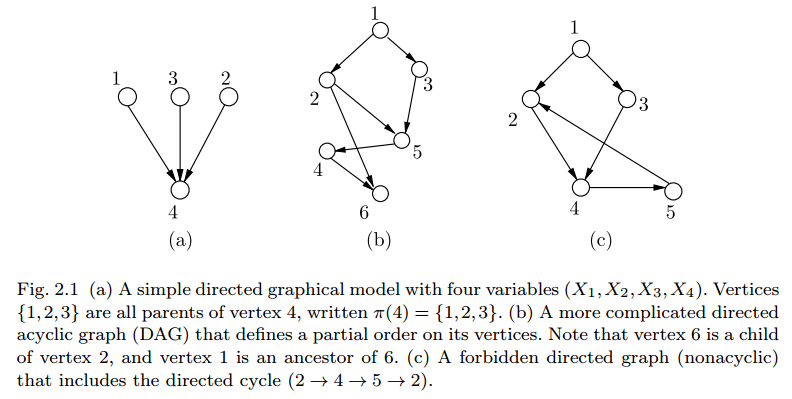
\includegraphics[scale = 0.45]{directed_graphical_model_ordering.png}}
\end{minipage}
\caption{\footnotesize{\textbf{The directed graphical model and the ordering of its vertices based on directed edges.}}}
\label{fig: directed_graphical_model_ordering}
\end{figure}


\section{Probabilistic Graphical Models}
Given a graph $\cG = (\cV, \cE)$, where $\cV$ is the set of vertices and $\cE \subset \cV \times \cV$ is the set of edges, a \emph{probabilistic graphical model (PGM)} defines a \emph{joint probability distribution} $p(x_1, \ldots, x_{m})$ that \underline{\emph{\textbf{factorizes}}} according to $\cG$. Here each variable $x_i$ corresponds to a node $v_i \in \cV$ and the existence of an edge $(s,t) \in \cE$ (or the \emph{\textbf{absence}} of an edge $(s,t)$) defines a \textbf{statistical dependency} (or \underline{\textbf{conditional independency}}) relation between $x_s$ and $x_t$.  

In particular, according to the type of edges, we can define two different types of PGMs:

\subsection{Directed graphical models (Bayesian networks)} 
If the edge $(s, t) \in \cE$ is \textbf{directed} (referred $s\rightarrow t$), i.e. there is a distinction between $(s, t)$ and $(t, s)$, the corresponding graphical models are referred as \emph{{directed graphical models}}.  Note that since a sequence of directed edges defines a logic flow, a circle in the graph would create undesireable contradiction. Therefore, we assume that $\cG$ is a \textbf{directed acyclic graph (DAG)}, meaning
that every edge is directed, and that the graph contains no directed cycles. 

For any such DAG, we can define a \textbf{partial order} on the vertex set $\cV$ by the notion of \emph{ancestry}:  we say that node $s$ is an \emph{ancestor} of $u$ if there is a \emph{directed path} $(s,t_1,t_2,\ldots,t_k,u)$. This is referred as \textbf{\emph{topological ordering}}. Given a DAG, for each vertex $u$ and its parent set $\pi(u) = \set{s \in \cV: (s\rightarrow u) \in \cE }$, the conditional probability $p_s(x_s | x_{\pi(s)})$ is a \textbf{non-negative function} over $ (x_s, x_{\pi(s)})$ and is \textbf{normalized} for all $x_s$, i.e. $\int p_s(x_s | x_{\pi(s)}) dx_s = 1.$

The \textbf{directed graphical model} thus factorizes the joint distribution into a set of \emph{local functions} $\{p_s(x_s | x_{\pi(s)}): s\in \cV\}$ according to the ancestor relations defined in $\cG$
\begin{align}
p(x_1, \ldots, x_{m}) &= \prod_{s \in \cV}p_s(x_s | x_{\pi(s)}). \label{eqn: dag_graph_factorization}
\end{align} This class of models are also referred as \emph{\textbf{Bayesian networks}} \citep{koller2009probabilistic}.


\begin{figure}
\begin{minipage}[t]{1\linewidth}
  \centering
  \centerline{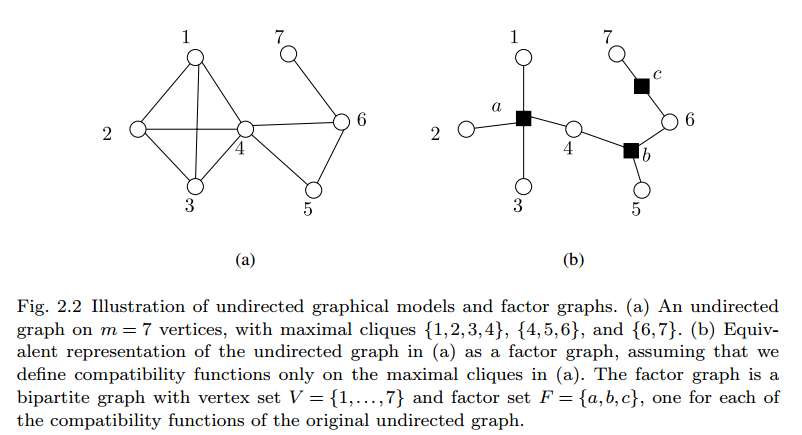
\includegraphics[scale = 0.45]{factor_graph.png}}
\end{minipage}
\caption{\footnotesize{\textbf{The undirected graphical model and its factor graph representation.}}}
\label{fig: factor_graph}
\end{figure}

\subsection{Undirected grapical models (Markov networks)}
In the \emph{undirected} case, the probability distribution factorizes according to functions defined on the \emph{\textbf{cliques}} of the graph. A clique $C$ is a \emph{\textbf{fully connected subset}} of the vertex set $\cV$ , meaning that $(s,t) \in \cE$ for all $s,t \in C$.
Let us associate with each clique $\cC$ a \emph{\textbf{compatibility function}} $\psi_{C}: (\otimes_{s\in C}\cX_{s}) \rightarrow \bR_{+}$, where $\otimes_{s\in C}\cX_{s}$ denotes the Cartesian product of the state spaces of the random vector $X_{C}$.  Consequently, the compatibility function $\psi_{C}$ is a local quantity, defined only for elements $x_C$ within the clique.

With this notation, an \emph{undirected graphical model} -- also known as a \emph{\textbf{Markov random field (MRF)}}, \emph{Markov Network}, or a \emph{Gibbs distribution} -- is a collection of distributions that \emph{factorize} as
\begin{align}
p(x_1, \ldots, x_{m}) &= \frac{1}{Z}\prod_{C \in \cC}\psi_{C}(x_{C}),\label{eqn: mrf_graph_factorization}
\end{align} where $Z$ is a constant chosen to ensure that the distribution is normalized. The set $\cC$ is often taken to be the \emph{set of all \textbf{maximal cliques} of the graph}, i.e., the set of cliques that are \emph{not} properly contained within any other clique. Note that any representation based on nonmaximal cliques can always be converted to one based on maximal cliques by redefining the compatibility function on a maximal clique to be the \emph{product} over the compatibility functions on the \emph{subsets} of that clique.


\subsection{Factor graph representation} 
To order to emphasize the computational structure and the factorization of dependencis, we introduce the \textbf{factor graph representation}. A factor graph is a \textbf{bipartite graph} $\cG' = (\cV, \cF, \cE')$ where $\cV$ is the same as the original graph. The set $\cF$ is the index set of \emph{factors}, e.g. the local functions for parent-child relationships or the compatibility function on cliques. $\cE'$ is a new edge set, joining only vertices $s \in  \cV$ to factors $a \in \cF$. In particular,
edge $(s,a) \in \cE$ if and only if $x_s$ \emph{participates} in the factor indexed by $a \in \cF$. Figure \ref{fig: factor_graph} shows the undirected graphical model and its factor graph representation.



\subsection{Important notes}
There are several important notes when learning graphical models:
\begin{itemize}
\item A probabilistic graphical model is a \underline{model \emph{\textbf{over}} graph $\cG$}, \textbf{not} a \underline{model \emph{\textbf{of}} graph $\cG$}. The latter is covered by \underline{\textbf{\emph{statistical network theory}}} \citep{goldenberg2010survey,  jackson2010social, newman2018networks}. The difference is that while the graph in PGM is used to model \underline{statistical} \underline{dependencies over variables} and to \underline{develop inference algorithms}, the sample data $\mb{X}_{i} := [X_{1,i}, \ldots, X_{m,i}]$ is still just a $m$-dimensional vector drawn i.i.d. from this distribution. On the other hand, a sample generated by a statistical network is a \textbf{graph itself}, i.e. $(\mb{X}_{i}, G_{i})$ a pair of \emph{node} samples, as well as graph topologies via \emph{edge} samples. Sometimes this graph-like sample is also referred as a \emph{\textbf{graph signal}} \citep{ortega2018graph}. The graph in PGM is a \textbf{\emph{structure} of models} and \textbf{computation} not an \textbf{observation}. The graph of PGM also does not reflect the topolocial dependencis between two variables in the observation but only its statistical dependencies. 

\item A \textbf{deep learning model} \citep{goodfellow2016deep} is a probabilistic graphical model with \textbf{\emph{hierarchical representation}}.  Unlike most of PGM we discussed, most of nodes of deep learning model represent \textbf{latent variables}, i.e. unobserved variables. These variables exist to decode the complicated relationship between observed input nodes. Deep learning models explore the \emph{overparameterized function space} in order to find suitable compatibility function $\psi$.

\item Given data samples, one need to first propose a graph representation of distribution before starting the inference and learning process. Usually, this graph comes from domain expertise. But most of time, it is unclear how to find a proper graph representation of the problem.  The \textbf{structural learning} of graphical models is very \textbf{challenging}. Unlike a \emph{deep learning model} which only cares for \underline{\emph{\textbf{function approximation}}}, a PGM cares if the graph structure indeed represents the \textbf{true underlyiing \underline{conditional independencies}}, which requires a series of testing. 
\end{itemize}

\subsection{Representation of factors}
\begin{figure}
\begin{minipage}[t]{1\linewidth}
  \centering
  \centerline{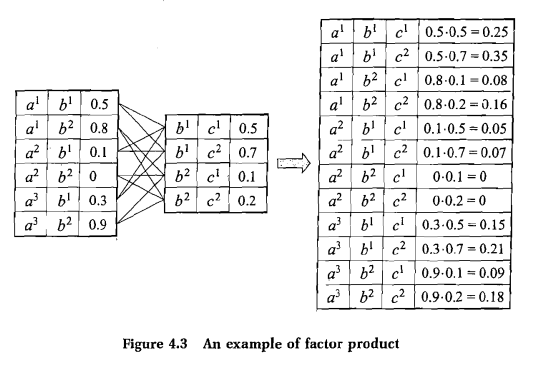
\includegraphics[scale = 0.45]{tab_factor.png}}
\end{minipage}
\caption{\footnotesize{\textbf{The tabular representation for each factor.}}}
\label{fig: tab_factor}
\end{figure}

A graphical model is a \emph{\textbf{\underline{distributed system}}}. \underline{\textbf{Factors}} are basic \textbf{building blocks} for graphical model. Since graphical models factorize over graph topology $\cG$, they store their \emph{information} \emph{locally} within  factors. Each factor covers a close \emph{neighborhood} of each node. For Bayesian networks, it is the \textbf{conditional probability}  $p_s(x_s | x_{\pi(s)})$ and for Markov random fields, it is the \textbf{compatiablity function} $\psi_{C}(x_{C})$ for each clique $C$. The \textbf{key idea} when learning graphical models is to understand how local information are \emph{\textbf{represented}}, \emph{\textbf{stored}} as well as to learn how they are \emph{\textbf{propagated}} across graph to obtain global information. 

\subsubsection{Tabular representation}
If the random variables are all \underline{\textbf{discrete with finite support}} and the \underline{\textbf{number}} of random variables involved in each \textit{factor} is small (like $2-4$), a tabular representation of these local factors are available. This requires that the underlining graph $\cG$ is \emph{\textbf{simple}} such as \emph{\textbf{tree}-structured} so that the  \underline{\textbf{size of neighborhood}} for a given node or a \underline{\textbf{clique}} is very small. Figure \ref{fig: tab_factor} shows a tabular form of factor product.

The advantages of tabular representation:
\begin{itemize}
\item \textbf{Simple and natural}: A table representation is natural and simple for many applications in statistics such as \emph{\textbf{contingency table analysis}}. For these applications, the multi-dimensional data forms a \textbf{high-dimensional tensor}, each storing the occurrence frequency of each \emph{possible outcome} under a set of configurations under many repeated experiments.

\item \textbf{Easy for parallel computation}: A key step in inference is to compute the \textbf{product of factors} (e.g. the \emph{marginalization}). Since each factor is represented by a tensor, this is simply a tensor product computation, which is easy to perform under parallel computing devices such as GPUs. Belief propagation also requires parallel computation during message passing. 

\item \textbf{Efficient inference}: Each factor is represented independently. This allows marginalization and maximization within each local factor. Tabular representation is suitable for efficient \emph{dynamic programming algorithms} such as \emph{\textbf{belief propagation}} (\emph{sum-product} and \emph{max-product}).

\item \textbf{High discrimination provides theoretical guarantee}: For each random variables, the frequence for each outcome is stored in table independently. Therefore, updating the probability value for one variable wil \emph{not affect} the probability of other variables. In other words,  random variables are fully discriminated in the table. This allows us to develop theories that prove the optimality with convergence guarantee. 
\end{itemize}

The disadvantages include
\begin{itemize}
\item \textbf{Not supporting continous variables}. Table can only represent discrete variables or discretized version of original function. Thus it easily introduces the quantization error in the process. 

\item \textbf{Not suitable for high dimensional factor}: Each factor in the table cannot be involve too many variables. Otherwise, the common operations within factors would be too costly. 

\item \textbf{High cost of storage} The size of tensor is determined by the \textbf{dimensionality} of factor as well as the \textbf{cardinality} of random variable domain. It can quickly explode when the graph is \emph{growing} and forms a \textbf{big clique}. This is typical in \emph{dynamic} graphical models. 
\end{itemize}

\subsubsection{Function approximation}
The factors can be represented via \textbf{parameterization}: $\mb{\eta} \rightarrow \psi_{\mb{\eta}}$. There are mainly two ways: the \emph{exponential family}, which is essentially \textbf{linear mapping}, and the \emph{deep neural network}, which is overparameterized \textbf{nonlinear mapping}. 
\begin{itemize}
\item  The commonly used function representation for distributions are the exponential famlity. The joint distribution $p(\mb{x})$ follows the canonical form \underline{\emph{\textbf{exponential famlity}}} of distribution
\begin{align}
p(x_1, \ldots, x_{m}) = p(\mb{x}; \mb{\eta}) &= \exp\paren{\inn{\mb{\eta}}{\mb{\phi}(\mb{x})} - A(\mb{\eta})}h(\mb{x})\nu(d\mb{x}) \nonumber \\
&= \exp\paren{\sum_{\alpha}\eta_{\alpha}\phi_{\alpha}(\mb{x}) -  A(\mb{\eta})}h(\mb{x})\nu(d\mb{x}) \label{eqn: exp_fam}
\end{align} where $\phi$ is a feature map  and $\mb{\phi}(\mb{x}_{C})$ defines a set of \emph{\textbf{sufficient statistics}} (or \emph{\textbf{potentials}}). The normalization factor is defined as
\begin{align*}
 A(\mb{\eta}) &:= \log \int \exp\paren{ \inn{\mb{\eta}}{\mb{\phi}(\mb{x})} }h(\mb{x})\nu(d\mb{x}) = \log Z(\mb{\eta})
\end{align*} $A(\mb{\eta})$ is also referred as \textbf{\emph{log-partition function}} or \emph{cumulant function}. The parameters $\mb{\eta} = (\eta_{\alpha})$ are called \textbf{\emph{natural parameters}}  or \emph{canonical parameters}. $\mb{\eta} \in \{\mb{\eta} \in \bR^{d}: A(\mb{\eta}) < \infty\}$, which is called \emph{natural parameter space}. Note that $A(\mb{\eta})$ is a convex function. 

In exponential family, due to property of exponent, we can formulate the (unnormalized) local functions as a exponential family too
\begin{align*}
\phi_{C}(\mb{x}_{C}; \mb{\eta}_{C}) &= \exp\paren{\sum_{k_{C}}\eta_{k_{C}}\phi_{k_{C}}(\mb{x}_{C})}
\end{align*}

Commonly known distribution and there natural parameterization:
\begin{itemize}
\item Bernoulli distribution $\text{B}(x; p)$: $\nu = \text{Counting measure}$,  $\eta = \log(p/(1-p))$, $\phi(x) = x$
\begin{align*}
\inn{\eta}{\phi(x)} &= \log\paren{\frac{p}{1-p}}x\\
A(\eta) &=-\log(1-p) =  \log(1 + \exp(\eta))  
\end{align*}

\item Gaussian distribution $\cN(\mb{x}; \mb{\mu}, \mb{\Sigma})$: $\nu = \text{Lebesgue measure } \bR^d$, $h(\mb{x}) = \frac{1}{(2\pi)^d}$, 
\begin{align}
\mb{\eta} &= \paren{\mb{\Sigma}^{-1}\mb{\mu}, - \frac{1}{2} \text{vec}(\mb{\Sigma}^{-1})} : = \paren{\mb{\theta}, -\frac{1}{2}\text{vec}(\mb{\Theta})} \label{eqn: gaussian_natural_param}\\
\mb{\phi}(\mb{x}) &= (\mb{x}, \text{vec}(\mb{x}\mb{x}^{T}))  \label{eqn: gaussian_sufficient_stats}\\
\inn{\mb{\eta}}{\mb{\phi}(x)} &= \mb{x}^{T}\mb{\Sigma}^{-1}\mb{\mu} - \frac{1}{2}\mb{x}^{T}\mb{\Sigma}^{-1}\mb{x} = \mb{x}^{T}\mb{\theta} - \frac{1}{2}\mb{x}^{T}\mb{\Theta}\mb{x} \nonumber\\
A(\mb{\eta}) &= \frac{1}{2}\paren{\mb{\mu}^{T}\mb{\Sigma}^{-1}\mb{\mu} + \log \det\abs{\mb{\Sigma}}} = \frac{1}{2}\paren{\mb{\theta}^{T}\mb{\Theta}^{-1}\mb{\theta} - \log \det\abs{\mb{\Theta}}}  \label{eqn: gaussian_partition_fun}
\end{align}

\item Poisson distribution $\text{Possion}(\lambda)$: $\nu = \text{Counting measure}$ $h(x) = 1/(x!)$, $\eta =  \log(\lambda)$, $\phi(x) = x$
\begin{align*}
\inn{\mb{\eta}}{\mb{\phi}(x)} &= \log(\lambda)x \\
A(\eta) &=\lambda =  \exp(\eta)
\end{align*}

\item Gamma distribution $\Gamma(\alpha, \lambda)$: $\nu = \text{Lebesgue measure } (0,\infty)$, $\mb{\eta} = (-\lambda, \alpha - 1)$  and $\mb{\phi}(x) = (x, \log(x))$
\begin{align*}
\inn{\mb{\eta}}{\mb{\phi}(x)} &= -\lambda x + (\alpha - 1)\log(x)  \\
A(\eta) &=\log(\Gamma(\alpha)) - \alpha \log(\lambda) = \log(\Gamma(\eta_2 + 1)) - (\eta_2 + 1) \log(-\eta_1) 
\end{align*}
\end{itemize}


\item We can \emph{re-parameterize} the exponential family by choosing mean parameter $\mb{\theta}$ as parameter when $\mb{\eta}:= \mb{\eta}(\mb{\theta})$. In \eqref{eqn: exp_fam}, if $\mb{\eta}:= \mb{\eta}(\mb{\theta}) = \mb{\theta}$, we call it canonical form. 
\begin{align}
p(x_1, \ldots, x_{m}) = p(\mb{x}; \mb{\theta}) &= \exp\paren{\inn{\mb{\eta}(\mb{\theta})}{\mb{\phi}(\mb{x})} - A(\mb{\eta}(\mb{\theta}))} \nonumber \\
&= \exp\paren{\sum_{\alpha}\eta_{\alpha}(\mb{\theta})\phi_{\alpha}(\mb{x}) -  A(\mb{\eta}(\mb{\theta}))} \label{eqn: exp_fam_natural}
\end{align}
From \citep{wainwright2008graphical} we can see that the form in \eqref{eqn: exp_fam} and \eqref{eqn: exp_fam_natural} are both \emph{\textbf{conjugate}} to each other based on convex analysis.


\begin{itemize}
\item A special form of exponential family is the \emph{\textbf{generalized linear models (GLMs)}}, when $p(x_s | x_{C})$ follows exponential family, $\phi(\mb{x}) = \inn{\mb{\theta}}{\mb{x}}$, 
\begin{align}
\mb{\mu} = \E{\mb{\eta}}{\mb{\phi}(\mb{x})} &= g^{-1}\paren{ \inn{\mb{\theta}}{\mb{x}}} \label{eqn: glm}
\end{align} where $g$ is called the \emph{\textbf{link function}}, $\inn{\mb{\theta}}{\mb{x}}$ is referred as linear predictor or system components. $g= (\grad{}{A})^{-1}$ where $A(\mb{\eta})$ is the log-partition function.
\end{itemize}

\item The other way to parameterize the local function is via \underline{\textbf{\emph{deep neural network}}}. See \citep{bengio2009learning, goodfellow2016deep, kingma2019introduction} for detailed discussion on neural networks.
\begin{align}
p_s(\mb{x}_s | \mb{x}_{\pi(s)}) &:= p_s(\mb{x}_s | \mb{\eta}) \nonumber\\
\text{where } \mb{\eta}&= \text{deep-net}( \mb{x}_{\pi(s)}).  \label{eqn: fun_approx_deep_net}
\end{align}
\end{itemize}

Compare to tabular representation, the function approximation has several advantages:
\begin{itemize}
\item \textbf{Efficient factor representation}: compare to the size of tensor for each factor, the parameterized function just need to maintain its parameter, which is much less compared to the dimensionality and cardinality of random vectors. 

\item \textbf{Support continuous variables}: Tabular representation is not for continous variables. For parameterized function approximator, one can build factors using continous input. 

\item \textbf{Convex analysis}: Learning exponential families involves solving \textbf{convex optimization} problems. The concept of \emph{conjugate duality} allows us to formulate it as \emph{maximum entropy estimation}. The \emph{smoothness} of \emph{log-partition function}, its \emph{variational form} via \emph{negative entropy function} and its gradient map etc. provide critical tools to analyze and develop efficient \emph{variational inference} algorithms with convergence guarantee.

\item \textbf{Universal function approximator}: Using simple nonliner functions, one can build a complex network that are capable of representing any functions. This is an important theorem behind the \emph{artificial neural networks} which is a type of graphical model (with hierarchical bipartite graph) using simple non-linear function to approximate factors. 
\end{itemize}

The disadvantages are
\begin{itemize}
\item \textbf{Integration results lack explicit forms}. \emph{Integration} over a large space is required for tasks such as  \emph{margalization}, the \emph{log-partition function} $A$ and the \emph{entropy function} $-A^{*}$ etc. Except for a few cases, the result of integration in general graphical model cannot be represented in \textbf{explicit function form}.  \emph{Approximation} via \textbf{\emph{Monte Carlo sampling methods}} (such as \emph{MCMC, Gibbs sampling}) \citep{shapiro2003monte} has been introduced. The other way is via \textbf{\emph{variational methods}}. Finally, one can rely on auto-differentiation such as the \emph{\textbf{backpropagtion}} to find local optimal solution for inference.

\item \textbf{Approximate inference}: Graphical models such as exponential families are defined using joint distributions. Both the log-partition function $A$ and the negative entropy function $A^{*}$ lack of explicit form. Moreover, they are not decomposable according to graph topology $\cG$.  This makes inference algorithms such as belief propagation very difficult to implment. One has to rely on \emph{variational methods} to \textbf{approximate} the objective functions, adding additional apprximation errors. 

\item \textbf{Loss global convergence}: Many variational methods are \textbf{non-convex} at the expense of being decomposable according to graph. These methods can only reach to local optima.

\item \textbf{Generalization vs. discrimination}. Using function means that the update of one probabilty value will affect the other probability value when all of them share the same sufficient statistics. This makes it hard to implement iterative algorithms that based on the local graph topology.
\end{itemize}


\newpage
\section{Conditional independence}
The most important property in graphical models is the \textbf{\emph{Markov properties}} over graph. In particular, let $A$, $B$, and $S$ be an arbitrary triple of mutually disjoint subsets of vertices. Let us stipulate that $X_A$ be \textbf{\emph{conditional independent}} of $X_B$ given $X_S$,  denoted as $X_{A} \indep X_{B} | X_{S}$,  if there is \underline{\textbf{no path}} from a vertex in $A$ to a vertex in $B$ when we  \underline{\textbf{remove}} the vertices $S$ from the graph. The set $S$ is referred as \textbf{\emph{cut-set}}, and we say that node set $A$ and $B$ are \textbf{seperated} given $S$, denoted as $\text{sep}_{\cG}(A; B | S)$  \citep{koller2009probabilistic}. The \textbf{Markov property} over graph $\cG$ is written as 
\begin{align*}
p(x_{A} | x_{S}, x_{B}) = p(x_{A} | x_{S})\quad \text{ if }\text{sep}_{\cG}(A; B | S)
\end{align*} For directed graph, the definition of path is replaced by the notion of \emph{active trail}, which not only consider directed path from $A \leftrightarrow B$ but also that of a \emph{$v$-structure} $X_{i-1} \rightarrow X_{i} \leftarrow X_{i+1}$, when $X_i$ or one of its descendant is in $S$. See Figure \ref{fig: cond_indep} for illustration of the active trails (a path of all dependent variables). The existence of \textbf{v-structure dependency} indicates that sometimes dependent variables may not directly related but may related to a common variables. This is the effect of "\textbf{explaining away}". (like "an increase in activation of Earthquake leads to a decrease in activation of Burglar") Using this, for directed graph we have concept of $d$-separation \citep{koller2009probabilistic}.

\begin{figure}
\begin{minipage}[t]{0.5\linewidth}
  \centering
  \centerline{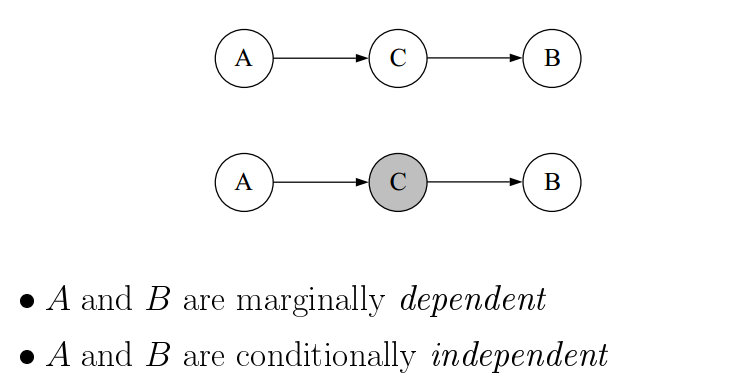
\includegraphics[scale = 0.32]{cond_indep_1.png}}
  \vspace{-5pt}
  \centerline{(a)}
\end{minipage}
\begin{minipage}[t]{0.5\linewidth}
  \centering
  \centerline{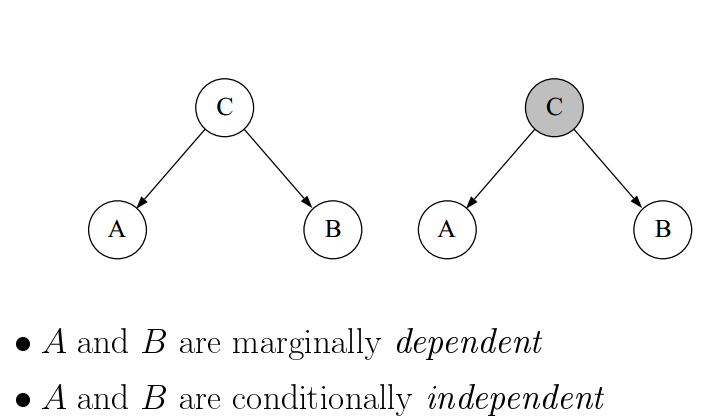
\includegraphics[scale = 0.3]{cond_indep_2.png}}
  \vspace{-5pt}
  \centerline{(b)}
\end{minipage}\\
\begin{minipage}[t]{0.5\linewidth}
  \centering
  \centerline{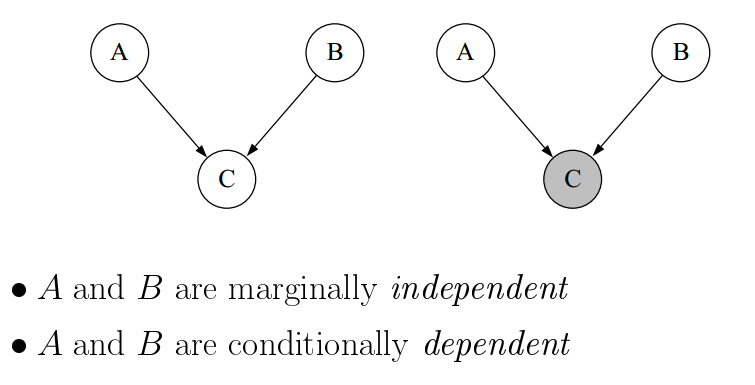
\includegraphics[scale = 0.35]{cond_indep_3.png}}
  \vspace{-5pt}
  \centerline{(c)}
\end{minipage}
\caption{\footnotesize{\textbf{The conditional independency structure in directed graph. The shaded nodes are observed. In (c), the variable $A$ and $B$ are marginally \emph{dependent} but conditionally \emph{independent}. }}}
\label{fig: cond_indep}
\end{figure}



For undirected graphical models, the \emph{\textbf{conditional independency}} is \emph{equivalent} to \emph{\textbf{graph reachability}}.  This equivalence is a fundamental mathematical result, linking an algebraic concept (\textbf{factorization}) and a graph-theoretic concept (\textbf{reachability}). This result also has algorithmic consequences, in that it reduces the problem of \emph{assessing conditional independence} to the problem of \emph{assessing reachability} on a graph, which is readily solved using simple breadth-first search algorithms.

Note that graphical model reprsentation is \textbf{not unique} since different models may represent the same set of conditional independence assertions among variables (i.e. \textbf{I-equivalence}). I-equivalence of two graphs immediately implies that any distribution $P$ that can be factorized over one of these graphs can be factorized over the other. This observation has important implications with respect to our ability to determine the directionality of influence (i.e. the direction of an edge $X\rightarrow Y$ or $X\leftarrow Y$). The direction can only be inferred via \textbf{causal analysis}.

Some useful properties for conditional independency:
\begin{itemize}
\item The set of neighbors is the separation set of a singular node
\begin{align*}
X \indep Y \,|\,  (\cV - \set{X, Y}) \\
X \indep (\cV -\set{X} -\cN_{\cG}(X)) \, |\, \cN_{\cG}(X)
\end{align*} where $\cN_{\cG}(X)$ is the set of all neighboring nodes of $X$ in the graph.

\item \textbf{Symmetry}: 
\begin{align*}
(X \indep Y \,|  Z) \Leftrightarrow (Y  \indep X  \,| Z).  
\end{align*}

\item \textbf{Decomposition}: 
\begin{align}
(X \indep (Y, W) \,|  Z) \Rightarrow (X  \indep Y  \,| Z).  \label{eqn: decomp}
\end{align}

\item \textbf{Weak Union}: 
\begin{align}
(X \indep (Y, W) \,|  Z) \Rightarrow (X  \indep Y  \,| (Z, W)).  \label{eqn: weak_union}
\end{align} Addition evidence from a conditional independent factor will not change the existing conditional independency with other factors.

\item \textbf{Contraction}: 
\begin{align}
(X \indep W \,| (Y, Z))\, \land \, (X \indep Y \,|  Z)  \Rightarrow (X \indep (Y, W) \,|  Z) .  \label{eqn: contraction}
\end{align} 

\item \textbf{Strong Union}: 
\begin{align}
(X \indep Y \,|  Z) \Rightarrow (X  \indep Y  \,| (Z, W)).  \label{eqn: strong_union}
\end{align} In other words, additional evidence $W$ cannot induce dependence.

\item \textbf{Transitivity}: For all disjoint sets $X$, $Y$, $Z$ and all variables $A$:
\begin{align}
\neg (X \indep A \,|  Z) \; \land\; \neg (A \indep Y \,|  Z)\; \Rightarrow \;\neg (X \indep Y \,|  Z)  \label{eqn: transitivity}
\end{align} Intuitively, this statement asserts that if $X$ and $Y$ are both correlated with some $A$ (given $Z$), then they
are also correlated with each other (given $Z$). We can also write the \textbf{contrapositive} of this statement,
which is less obvious but easier to read. For all $X$, $Y$, $Z$, $A$:
\begin{align}
 (X \indep Y \,|  Z)  \Rightarrow (X \indep A \,|  Z)\;  \lor \; (A \indep Y \,|  Z)   \label{eqn: transitivity_counterpositive}
\end{align}
\end{itemize}
\newpage
\section{Examples}
\subsection{Ising Models (binary Markov random field)}
\begin{figure}
\begin{minipage}[t]{1\linewidth}
  \centering
  \centerline{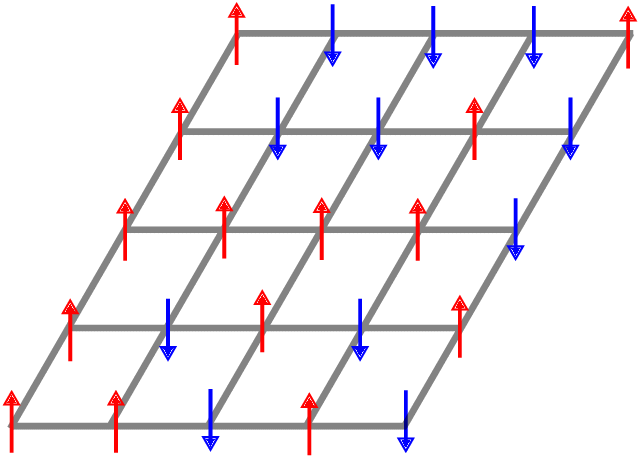
\includegraphics[scale = 0.3]{Ising_model.png}}
\end{minipage}
\caption{\footnotesize{\textbf{The Ising model which is built on a grid graph.}}}
\label{fig: Ising_model}
\end{figure}
The \textbf{\emph{Ising model}} from statistical physics is a classical example of a graphical model in exponential form. Consider a graph $\cG = (\cV,\cE)$ and suppose that the random variable $X_s$ associated with node $s \in \cV$ is \emph{\textbf{Bernoulli}}, say taking the “spin” values $\{-1,+1\}$.  In the context of statistical physics, these
values might represent the \emph{orientations} of magnets in a field, or the \emph{presence/absence} of particles in a gas. The Ising model and variations on it have also been used in image processing and spatial statistics.

Ising model is a \textbf{\emph{pairwise Markov random field}}. Its factors involve at most two variables. Therefore, its underlying is graph is usually a grid network. Ising model is a part of exponential family 
\begin{align}
p(x_1, \ldots, x_m) &= \exp\paren{\sum_{s\in \cV}w_s\,x_s + \sum_{(s,t) \in \cE}w_{s,t}\,x_s\,x_t - A(\mb{w})}, \label{eqn: ising_model}
\end{align} where the base measure $\nu$ is the counting measure restricted to $\{0,1\}^m.$ Here $w_{s,t} \in \bR$ is the \emph{strength} of edge $(s,t)$, and $w_s \in \bR$ is a \emph{potential} for node $s$, which models an "external field" in statistical physics, or a noisy observation in spatial statistics. Strictly speaking, the family of
densities \eqref{eqn: ising_model} is more general than the classical Ising model, in which $w_{s,t}$ is constant for all edges. The log-parition function 
\begin{align*}
A(\mb{w}) &= \log \sum_{\mb{x} \in \{0,1\}^m}\exp\paren{\sum_{s\in \cV}w_s\,x_s + \sum_{(s,t) \in \cE}w_{s,t}\,x_s\,x_t}
\end{align*}

Note that the local function (factor) is of the form
\begin{align*}
\phi_{s}(x_s, x_{\cN(s)}) &=  \exp\paren{w_s\,x_s + \sum_{t\in \cN(s)}w_{s,t}\,x_s\,x_t}
\end{align*} 

\subsubsection{Metric Labeling and Potts Model}
Consider a generalization of the Ising model: suppose that the random variable $X_s$ at each node $s \in \cV$ takes values in the \textbf{discrete space} $\cX := \{0,1, \ldots, r-1\}$, for some integer $r > 2$. One interpretation of a state $j \in \cX$ is as a label, for instance defining membership in an image segmentation problem. Each pairing of a node $s \in \cV$ and a state $j \in \cX$ yields a sufficient statistic 
\begin{align}
\phi_{s;j}(x_s) &= \ind{x_s = j}  \label{eqn: metric_label_sufficient}
\end{align} 
Moreover, for each edge $(s,t)$ and pair of values $(j,k) \in \cX \times \cX$ , define the sufficient statistics
\begin{align}
\phi_{st;jk}(x_s, x_t) &= \ind{x_s = j \, \land x_{t} = k}  \label{eqn: metric_label_sufficient2}
\end{align} Note that $\sum_{j\in \cX}\phi_{s;j}(x_s) = 1$.  Similar to \eqref{eqn: ising_model}, we have 
\begin{align}
p(x_1, \ldots, x_m) &= \exp\paren{\sum_{s\in \cV}\sum_{j \in \cX}w_{s;j}\,\phi_{s;j}(x_s)  + \sum_{(s,t) \in \cE}\sum_{(j,k) \in \cX \times \cX}w_{st;jk}\,\phi_{st;jk}(x_s, x_t)  - A(\mb{w})}, \label{eqn: potts_model}
\end{align} 

When $\phi_{st;jk}(x_s, x_t) :=- \rho(j, k)$ for some metric function $\rho: \cX \times \cX \rightarrow \bR_{+}$, we have the \textbf{\emph{metric labeling problem}}. Consequently, the canonical parameters satisfy the relations $w_{st;kk} = 0$ for all $k \in \cX$ , $w_{st;jk} < 0$ for all $j \neq k$, and satisfy the \emph{reversed triangle inequality} (that is, $w_{st;jl} \ge w_{st;jk} + w_{st;kl}$ for all triples $(j, k, l)$).  Another special case is the \textbf{\emph{Potts model}} from statistical physics, in which case $w_{st;kk} = \alpha$ for all for all $k \in \cX$ , and $w_{st;jk} = \beta$ for all $j \neq k$,.

The local function (factor) is of the form
\begin{align*}
\phi_{s}(x_s, x_{\cN(s)}) &=  \exp\paren{\sum_{j \in \cX}w_{s;j}\phi_{s;j}(x_s) + \sum_{t\in \cN(s)}\sum_{(j,k) \in \cX \times \cX}w_{st;jk}\,\phi_{st;jk}(x_s, x_t)}
\end{align*} 

\subsection{Gaussian graphical models (GGM)}
\begin{figure}
\begin{minipage}[t]{1\linewidth}
  \centering
  \centerline{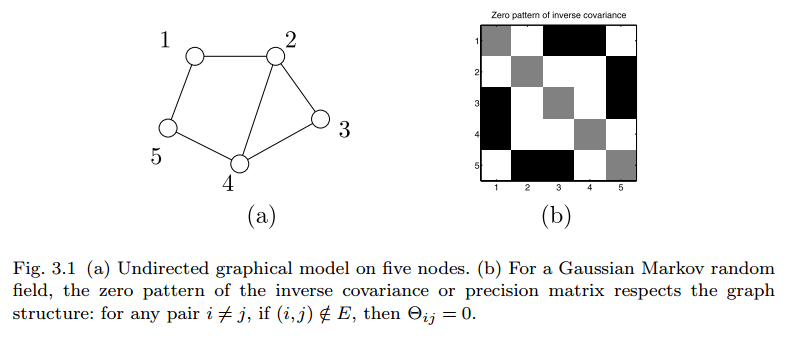
\includegraphics[scale = 0.45]{ggm.png}}
\end{minipage}
\caption{\footnotesize{\textbf{The Gaussian graphical model on undirected graph.}}}
\label{fig: ggm}
\end{figure}
Given an \emph{undirected} graph $\cG$ with vertex set $\cV = \{1,\ldots,m\}$, a \emph{Gaussian Markov random field (GMRF)} (or \emph{Gaussian graphical models}) \citep{wainwright2008graphical} consists of a multivariate \emph{Gaussian} random vector $(X_1,\ldots,X_m)$ that respects the Markov properties of $\cG$. It can be
represented in exponential form using the collection of sufficient statistics $\mb{\phi}(\mb{x}): = (x_s, x_s^2, s \in \cV; \; x_s\,x_t, \, (s,t) \in \cE)$. We define the inverse of covariance matrix $\mb{\Theta} = \mb{\Sigma}^{-1}$, which is referred as \textbf{precision matrix}. 

A \textbf{key property} that distinguishes Gaussian graphical model from other models is that the \textbf{\underline{\emph{graph structure}} is fully encoded in the \underline{\emph{precision matrix}}} $\mb{\Theta}$. That is, 
\begin{align}
(s,t) \not\in \cE\, \Leftrightarrow \,X_s \indep X_t | X_{\cV-\{s,t\}}\; \Leftrightarrow \; \mb{\Theta}_{s,t} = 0 \label{eqn: gaussian_cond_indep_precision}
\end{align}

 As shown in \eqref{eqn: gaussian_natural_param} and \eqref{eqn: gaussian_sufficient_stats},  the form of Gaussian graphical model is
\begin{align}
 p(\mb{x}; \mb{\theta}, \mb{\Theta}) &= \exp\paren{\inn{\mb{\theta}}{\mb{x}} - \frac{1}{2}\inn{\mb{\Theta}}{\mb{x}\mb{x}^{T}} - A(\mb{\theta}, \mb{\Theta})} \label{eqn: ggm_exp}
\end{align} Note that $\inn{\mb{\Theta}}{\mb{x}\mb{x}^{T}} := \text{tr}(\mb{\Theta}\mb{x}\mb{x}^{T})$ is the inner product btw matrices. The natural parameter space 
\begin{align}
\Omega = \set{\mb{\Theta} \in \text{Sym}_{m}, \mb{\theta} \in \bR^{m},    \mb{\Theta} \succ \mb{0}\;  }
\end{align}
Unlike most of graphical models,  the \textbf{log-partition function} of GGM has \textbf{closed-form}
\begin{align}
A(\mb{\theta}, \mb{\Theta}) &= \frac{1}{2}\paren{\mb{\theta}^{T}\mb{\Theta}^{-1}\mb{\theta} - \log \det\abs{\mb{\Theta}}}
\end{align} 

Another important property for Gaussian graphical model is that the \underline{\textbf{conditional distribution}} $p_s(\mb{x}_{S} | \mb{x}_{\cN})$, i.e. the \textbf{local function}, is also \underline{Gaussian distributed}
\begin{align}
p_s(\mb{x}_{S} | \mb{x}_{\cN})  &= \exp\paren{\inn{\mb{\theta}_{S| \mb{x}_{\cN}}}{\mb{x}_{S}} -  \frac{1}{2}\inn{\mb{\Theta}_{S}}{\mb{x}_{S}\mb{x}_{S}^{T}} - A(\mb{\theta}_{S| \mb{x}_{\cN}}, \mb{\Theta}_{S}) } \\
\text{where } \mb{\theta}_{S| \mb{x}_{\cN}} &=\mb{\Theta}_{S}\mb{\mu}_{S|\mb{x}_{\cN}} = \mb{\theta}_{S} -  \mb{\Theta}_{S, \cN}\mb{x}_{\cN}  \nonumber\\
\mb{\Theta} &=\brac{\begin{array}{cc}
\mb{\Theta}_{S} & \mb{\Theta}_{S, \cN}\\
\mb{\Theta}_{\cN, S} & \mb{\Theta}_{\cN,\cN}\\
\end{array}}
\end{align} where $S$ is the clique and $\cN = \cV - S$ is the complentary set to $S$, $\mb{\Theta}_{S}$ is the diagonal block of precision matrix $\mb{\Theta}$ corresponding to $S$. $\mb{\theta}_{S}$ is the $S$ block in $\mb{\theta}$.
Also 
\begin{align}
p_s(\mb{x}_{S} | \mb{x}_{\cN}) &= \cN(\mb{\mu}_{S| \mb{x}_{\cN}}, \mb{\Sigma}_{S| \cN}) \nonumber \\
\text{where }\mb{\mu}_{S|\mb{x}_{\cN}} &= \mb{\mu}_{S} + \mb{\Sigma}_{S, \cN}\mb{\Sigma}_{\cN}^{-1}(\mb{x}_{\cN} - \mb{\mu}_{\cN}) \label{eqn: guassian_conditional_mean}\\
&=  \mb{\mu}_{S} -   \mb{\Theta}_{S}^{-1}\mb{\Theta}_{S, \cN}(\mb{x}_{\cN} - \mb{\mu}_{\cN}) \nonumber\\
\mb{\theta}_{S} &= \mb{\Theta}_{S}\mb{\mu}_{S} + \mb{\Theta}_{S, \cN}\mb{\mu}_{\cN} \nonumber\\
\mb{\Sigma}_{S| \cN} &= \mb{\Sigma}_{S} - \mb{\Sigma}_{S, \cN}\mb{\Sigma}_{\cN}^{-1}\mb{\Sigma}_{\cN, S} \nonumber\\
 &= \mb{\Theta}_{S}^{-1}  \label{eqn: guassian_conditional_covariance}
\end{align}

Because of \eqref{eqn: gaussian_cond_indep_precision}, \underline{\textbf{parameter estimation}} in Gaussian graphical model with sparse regularization is equivalent to \underline{\textbf{structure learning}}, i.e. learning the underlying graph $\cG$ itself. Efficient \textbf{\emph{sparse inverse covariance estimation}} methods such as \emph{\textbf{Graphical Lasso}}, \emph{neighborhood regression} etc. \citep{wainwright2019high} are available for estimating the graph structure.


\subsection{Hidden Markov Chain (HMM)}
\begin{figure}
\begin{minipage}[t]{1\linewidth}
  \centering
  \centerline{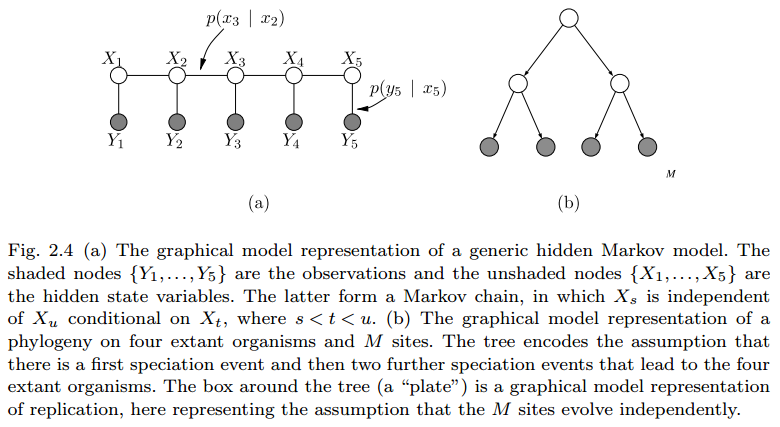
\includegraphics[scale = 0.45]{hmm.png}}
\end{minipage}
\caption{\footnotesize{\textbf{The Hidden Markov chain on directed chain graph is a generative model.}}}
\label{fig: hmm}
\end{figure}

The \textbf{\emph{hidden Markov model (HMM)}} is a \emph{generative} \emph{\textbf{Bayesian network}} on a directed chain-structured graph. Due to its simple structure, it is widely used in \emph{\textbf{sequential modeling}} such as \emph{part-of-speech tagging}, \emph{name entity recognition} in natural language processing, speech recognition, \emph{gene finding} in bioinformatics and \emph{decoding} in digital communications.

As a Bayesian network, HMM has two \emph{type} of nodes: the \emph{unobserved} one $\{x_t \in \cX\}_{t=1}^{T}$, referred as \textbf{state}, and the \emph{observed} one $\{y_t \in \cY\}_{t=1}^{T}$, referred as \textbf{observation}. The \textbf{state} variables are connected with each other via a \textbf{chain graph structure}, i.e. each state (except for initial state) has one and only one parent, and each observation only connect to one state. 

The size of \emph{state space} $r = |\cX|$ is usually \textbf{small}, and the \emph{state variables} are \textbf{discrete}. Therefore it is common to use the \textbf{tabular representation} to encode the HMM. Following Markov property, it is seen that HMM has \textbf{only two different local functions}: 
\begin{itemize}
\item The \textbf{\emph{state transition probabilty}} $p(x_{t}|x_{t-1})$. Let $\mb{P} = [p_{i,j}] = [p(x_{t}= j|x_{t-1} = i)] \in \bR^{|\cX| \times |\cX|}$

\item The \textbf{\emph{emission probability}} $p(y_t|s_{t})$. $\mb{B} = [b_{i}(y_t)] =  [p(y_t  | x_t = i)] \in \bR^{|\cY| \times |\cX|}$
\end{itemize} Note that these two functions are identical for all $t$. This is because the \emph{ergodic markov process} will reach steady-state in the long run, and at steady-state, the state transition probabilty  $p(x_t| x_{t-1}) = p(x_{t+1}| x_{t}) = \ldots$. This \emph{\textbf{recurrent structure}} allow HMM to cover sequences of different length.  
 
The joint distribution of \emph{HMM} is thus easy to follow
\begin{align}
p(x_0, x_1, \ldots, x_T ; y_1, \ldots, y_t) = \prod_{t=1}^{T}p(y_t | x_t)p(x_t| x_{t-1})p(x_{0})    \label{eqn: hmm}
\end{align}  

There are two tasks associated with HMM:
\begin{itemize}
\item \textbf{Inference} \emph{states} given observations: The inference in HMM is to find $x_{1:T}:= \{x_t\}_{t=1}^{T}$  that maximize the log-likehood function given observations $y_{1:T}:= \{y_t\}_{t=1}^{T}$
\begin{align}
\hat{x}_{1:T} &= \argmax_{x_{1:T}}p(x_{1:T} ; y_{1:T}) \nonumber\\
&=\argmax_{x_{1:T}} \prod_{t=1}^{T}p(y_t | x_t)p(x_t| x_{t-1})p(x_{0}) \label{eqn: hmm_inference}
\end{align} The algorithm to solve \eqref{eqn: hmm_inference} is based on \textbf{\emph{dynamic programming}}, called \textbf{\emph{Viterbi decoding}}. In particular, it utilizes the recursive structure of the model and defind the \emph{local objective} as \textbf{value function:}
\begin{align}
v_{t}(i) &:= \max_{x_{1:t-1}} p(x_{1:t-1}, o_{1:t-1}, x_t= i), \quad i =1,\ldots, r  \label{eqn: hmm_inference_value}
\end{align} It follows the following \textbf{Bellman equation} as recursion formula.
\begin{align}
v_{t}(i) &= \max_{j= 1,\ldots, r} v_{t-1}(j)\; p_{j,i}\; b_{i}(o_t), \quad i=1,\ldots, r  \label{eqn: hmm_inference_viterbi}
\end{align} This is essentially a \textbf{max-product algorithm}.

\item \textbf{Learning}, i.e. parameter estimation on $\mb{P}$ and $\mb{B}$: The estimation task for HMM need to find $\mb{P}$ and $\mb{B}$ that maximize the \textbf{marginalized likelihood function} over observation $y_{1:T}:= \{y_t\}_{t=1}^{T}$. Let $\mb{\theta}:= (\mb{P}, \mb{B})$
\begin{align}
\mb{\theta} &= \arg\max_{\mb{\theta}} p(y_{1:T} | \mb{\theta}) = \prod_{x_{1:T}}p(x_{1:T} ; y_{1:T} | \mb{\theta})
\end{align}
This is done via an \emph{\textbf{expectation-maximization (EM)}} algorithm called \textbf{\emph{Baum-Welch algorithm}}. Define the following quantities
\begin{align}
Q(\mb{\theta}, \mb{\theta}^{(l-1)}) &= \E{p(x_{1:T} |  y_{1:T}, \mb{\theta}^{(l-1)})}{\log p(x_{1:T} ; y_{1:T} | \mb{\theta})} \label{eqn: hmm_baum_welch_q}\\
\gamma_{i}(t) &= p(x_t = i | y_{1:T}, \mb{\theta}^{(l-1)})   \label{eqn: hmm_baum_welch_gamma}\\
\xi_{i,j}(t) &= p(x_{t} = i, x_{t+1} = j | y_{1:T}, \mb{\theta}^{(l-1)}) \label{eqn: hmm_baum_welch_xi}
\end{align} 

\begin{itemize}
\item \textbf{E-step}, i.e. estimation of $p(x_{1:T} |  y_{1:T}, \mb{\theta}^{(l-1)})$. This quantity can be split into two part at time $t$, one with past events and one with future events. Then we use the dynamic programming with a \textbf{forward-backward procedure}.
\begin{itemize}
\item \textbf{Forward step}: Define the \emph{forward value function} 
\begin{align}
\alpha_{i}(t) &:= p(y_{1:t}, x_t=i \,| \mb{\theta})   \label{eqn: hmm_baum_welch_alpha}
\end{align} That is the probability of observing \emph{past events} $y_{1},\ldots,  y_{t}$ \underline{\textbf{and}} being state $x_t=i$. This value function also has a \underline{\textbf{forward Bellman equation}}:
\begin{align}
\alpha_{i}(t+1) &= p(y_{t+1} | x_{t+1}=i)\sum_{j}p(x_{t+1} = i | x_{t}= j)\alpha_{j}(t)  \label{eqn: hmm_baum_welch_bellman}\\
&= b_{i}(y_{t+1})\sum_{j}p_{j,i}\alpha_{j}(t)  \nonumber
\end{align}

\item \textbf{Backward step}: Similarly, define the \emph{backward value function} 
\begin{align}
\beta_{i}(t) &:= p(y_{(t+1):T}\,|x_t=i, \mb{\theta})   \label{eqn: hmm_baum_welch_alpha}
\end{align} That is the probability of observing \emph{future} \emph{events} $y_{t+1},\ldots,  y_{T}$ \underline{\textbf{given}} state $x_t=i$. This value function also has a \underline{\textbf{backward Bellman equation}}:
\begin{align}
\beta_{i}(t) &= \sum_{j}p(x_{t+1} = j | x_{t}= i)p(y_{t+1} | x_{t+1}=j)\beta_{j}(t+1)  \label{eqn: hmm_baum_welch_bellman}\\
&= \sum_{j}p_{i,j}b_{j}(y_{t+1}) \beta_{j}(t+1) \nonumber
\end{align}
\end{itemize} This is essentially a \textbf{sum-product algorithm} to compute marginal distribution.

\item \textbf{M-step}, i.e. maximization of $\E{p(x_{1:T} |  y_{1:T})}{\log p(x_{1:T} ; y_{1:T} | \mb{\theta})}$. Update the $\gamma_{i}(t)$ and $\xi_{i,j}(t)$ via
\begin{align}
\gamma_{i}(t) &= \frac{\alpha_{i}(t)\beta_{i}(t)}{\sum_{j}\alpha_{j}(t)\beta_{j}(t)} \label{eqn: emission_update_local}\\
\xi_{i,j}(t) &= \frac{\alpha_i(t)\; p_{i, j}\, \;\beta_{j}(t+1)\,b_{j}(y_{t+1}) }{\sum_{k}\sum_{s}\alpha_k(t)\; p_{k, s}\, \;\beta_{s}(t+1)\,b_{s}(y_{t+1})}  \label{eqn: transition_update_local}
\end{align} 

Finally, the estimate $\hat{\mb{P}} = [\hat{p}_{i, j}]$ and $\hat{\mb{B}} = [\hat{b}_{j}(y)]$
\begin{align}
\hat{p}_{i, j} &= \frac{\sum_{t=1}^{T}\xi_{i,j}(t)}{\sum_{t=1}^{T}\gamma_{i}(t) }  \label{eqn: transition_update}\\
\hat{b}_{i}(y) &= \frac{\sum_{t=1}^{T}\ind{y_t = y}\gamma_{i}(t)}{\sum_{t=1}^{T}\gamma_{i}(t)} \label{eqn: emission_update}
\end{align}
\end{itemize}
\end{itemize}




\subsection{Conditional Random Field (CRF)}
\begin{figure}
\begin{minipage}[t]{1\linewidth}
  \centering
  \centerline{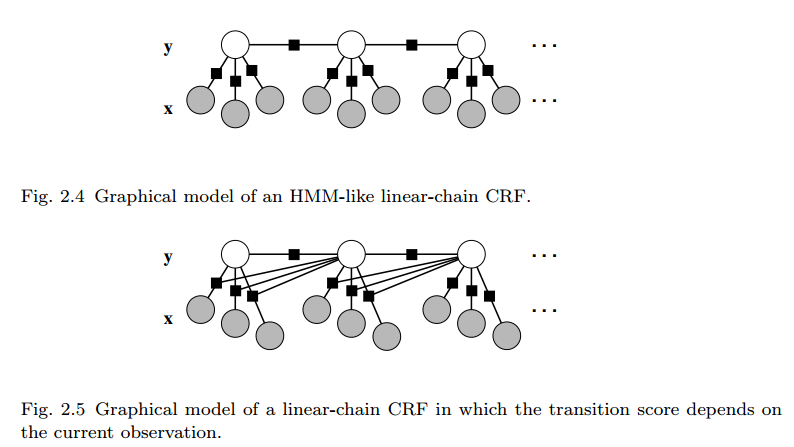
\includegraphics[scale = 0.5]{crf.png}}
\end{minipage}
\caption{\footnotesize{\textbf{Comparison of generative graphical models and discriminative graphical models \citep{sutton2012introduction} }.}}
\label{fig: crf}
\end{figure}

HMM is a generative model. It is hard for HMM to add arbitrary features directly into the model. A discriminative model can be better. The \textbf{conditional random field (CRF)} \citep{sutton2012introduction} can be used to solve this issue. The most commonly used CRF is linear chain CRF, which is close to HMM. Similar to HMM, CRF optimize the posterior probability
\begin{align*}
\hat{x}_{1:T} &= \argmax_{x_{1:T}} p(x_{1:T} | y_{1:T}).
\end{align*} Unlike HMM, CRF define the conditional probability directly as a \textbf{log-linear} model: 
\begin{align*}
p(x_{1:T} | y_{1:T}) &= \frac{1}{Z(y_{1:T})} \exp\paren{\sum_{k=1}^{K}w_{k}F_{k}(\mb{x}, \mb{y})}\\
&= \frac{1}{Z(y_{1:T})} \exp\paren{\sum_{k=1}^{K}\sum_{t}^{T}w_{k}f_{k}(x_{t}, x_{t-1}, y_{1:T}, t)}\\
\end{align*} Each $f_{k}$ is called a \textbf{local feature}, which is accumulated over time to form a \textbf{global feature} $F_{k}$. Each of local feature is a linear-chain CRF which makes use of the current state/tag $x_{t}$ and previous state/tag $x_{t-1}$ and the entire observations $y_{1:T}$ and the current position $t$. It is linear chain CRG since $f_{k}$ only depends on $x_{t}$ and $x_{t-1}$. An example pos feature $f_{k}:= \ind{y_{t} = \text{"the"}, x_{t} = \text{DET}}$ and 
$f_{s} := \ind{y_{t+1} = \text{"Street"}, x_{t}=\text{PROPN},  x_{t-1}=\text{NUM}}$. For NER feature, could be "identity of $y_{i}$, identity of neighboring words". 

The linear structure of CRF makes it easy to build \textbf{binary feature} and extend to different special cases. These feature can be manually designed or automatically generated via \textbf{feature templates}: $<x_{t}, y_{t}>, <x_{t}, x_{t-1}>, <x_{t}, y_{t-1}, y_{t+1}>$. These features can be generated from training data. For unknown words, we can define the \textbf{word shape} features, which represent the \emph{\textbf{abstract letter pattern}} of the word by mapping lower-case letters to ‘x’, upper-case to ‘X’, numbers to ’d’, and retaining punctuation, e.g. $I.M.F:= X.X.X$. Prefix and suffix features are also useful. For example some feature templates with unknown words such as "$y_i$ contains a particular prefix/suffix" or "$y_{i}$'s word shape" etc.

The \emph{known-word templates} are computed for every word seen in the training set; the \emph{unknown word features} can also be computed for all words in training, or only on training words whose frequency is below some threshold. The result of the known-word templates and word-signature features is \emph{a very large set of features}.

In NER, one feature that is especially useful for \textbf{locations} is a \textbf{gazetteer}, a list of place names, often providing millions of entries for locations with detailed geographical and political information. This can be implemented as a \textbf{binary feature} indicating a phrase appears in the list. Other related resources like name-lists can be used, as can other entity dictionaries like lists of corporations or products, although they may not be as helpful as a gazetteer

\subsection{Latent Dirichlet allocation (LDA)}
\begin{figure}
\begin{minipage}[t]{1\linewidth}
  \centering
  \centerline{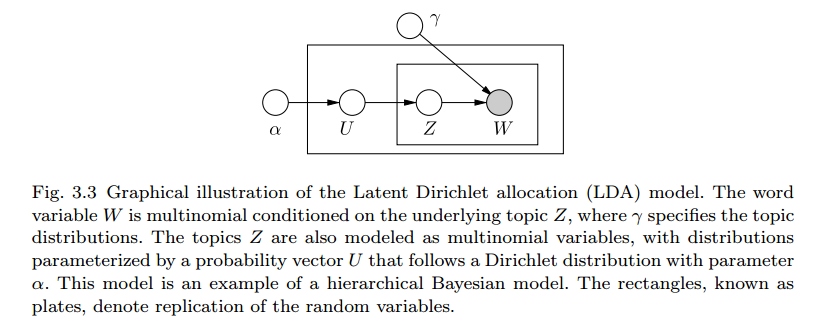
\includegraphics[scale = 0.45]{lda.png}}
\end{minipage}
\caption{\footnotesize{\textbf{The Latent Dirichlet allocation is a generative Bayesian network model.}}}
\label{fig: lda}
\end{figure}
The latent Dirichlet allocation model \citep{wainwright2008graphical} is a particular type of hierarchical Bayes model for capturing the statistical dependencies among words in a corpus of documents. It involves three different types of random variables: \emph{\textbf{documents}} $U$, \emph{\textbf{topics}} $Z$, and \emph{\textbf{words}} $W$. 

Words $W$ are drawn from a multinomial distribution, $p(W = j |Z = i; \gamma) = \exp(\gamma_{ij})$, for $j = 0,1,...,k − 1$, where $\gamma_{ij}$ is a parameter encoding the probability of the $j$-th word under the $i$-th \emph{topic}. This conditional distribution can be expressed as an \emph{exponential family} in terms of indicator functions as follows:
\begin{align}
p_{\gamma}(w|z) &\propto \exp\paren{\sum_{i=0}^{k-1}\sum_{j=0}^{r-1}\gamma_{ij}\ind{w=j}\ind{z=i}} \label{eqn: lda_words_per_topic}
\end{align} At the next level of the hierarchy (see FIgure \ref{fig: lda}) the topic variable $Z$ also follows a multinomial distribution whose parameters are determined by the \textbf{Dirichlet variable} as follows:
\begin{align}
p(z|u) &\propto \exp\paren{\sum_{i=0}^{k-1}\ind{z=i}\log(u_i)} \label{eqn: lda_topics_per_documents}
\end{align}
Finally, at the top level of the hierarchy, the \emph{\textbf{Dirichlet variable}} $U$ has a density with respect to Lebesgue measure of the
form 
\begin{align}
p_{\alpha}(u) &\propto \exp\paren{ \sum_{i=0}^{r-1}\alpha_{i} \log(u_i)}.
\end{align}

The overall joint distribution factorizes as below:
\begin{align}
p(w, z, u) &= p_{\gamma}(w|z) p(z|u) p_{\alpha}(u)  \nonumber\\
&\propto \exp\paren{ \sum_{i=0}^{r-1}\alpha_{i} \log(u_i) + \sum_{i=0}^{k-1}\ind{z=i}\log(u_i) + \sum_{i=0}^{k-1}\sum_{j=0}^{r-1}\gamma_{ij}\ind{w=j}\ind{z=i}} \label{eqn: lda}
\end{align} The sufficient statistics  consist of the collections of functions $$\mb{\phi}(w,z,u)= ((\log(u_i))_i, (\ind{z=i})_i, (\ind{w=j}\ind{z=i})_{i,j}).$$



\subsection{Restricted Boltzmann machine (RBM)}
\begin{figure}
\begin{minipage}[t]{0.5\linewidth}
  \centering
  \centerline{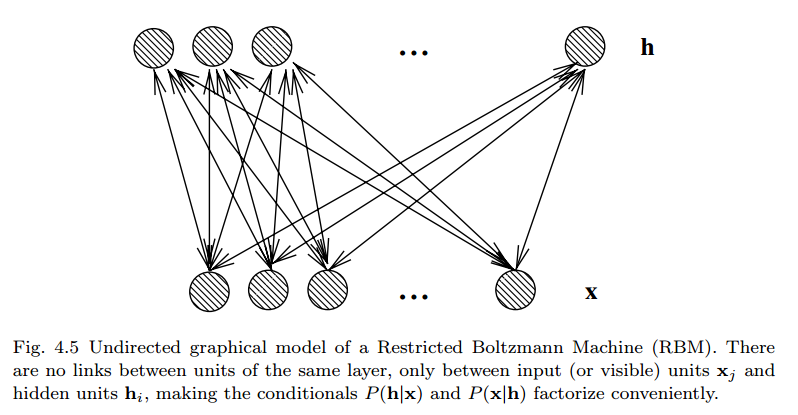
\includegraphics[scale = 0.3]{rbm.png}}
\end{minipage}
\begin{minipage}[t]{0.5\linewidth}
  \centering
  \centerline{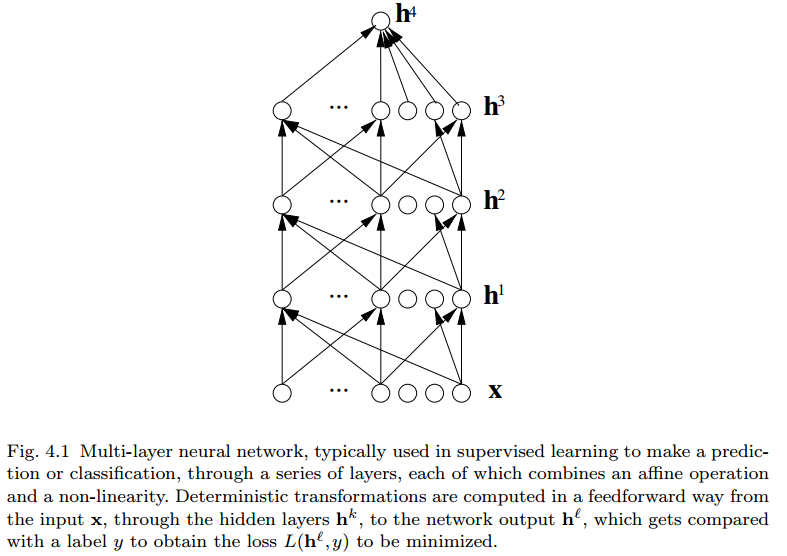
\includegraphics[scale = 0.3]{ffn.png}}
\end{minipage}
\caption{\footnotesize{\textbf{The restricted Boltzmann machine is a generative Bayesian model based on layerwise graph. \citep{bengio2009learning}
}}}
\label{fig: rbm}
\end{figure}

Traditionally, each conditional probability distribution $p_s(x_s | x_{\pi(s)})$ is represented by a tabular form or a linear model  \citep{koller2009probabilistic}. As we explained above, a more flexible way to parameterize such conditional distributions is with neural networks. 

For a \textbf{\emph{Deep Belief Network (DBN)}} with $l+1$ layers, the input observed variables are  denoted as $\mb{x}$, and the hidden variables at layer $k$ are denoted $\mb{h}^{(k)}$. The joint distribution is factorized as 
\begin{align}
p(\mb{x}, \mb{h}^{(1)}, \ldots, \mb{h}^{(l)}) &= p(\mb{x}|\mb{h}^{(1)})\paren{\prod_{k=1}^{l-2}p(\mb{h}^{(k)} | \mb{h}^{(k+1)})}p(\mb{h}^{(l-1)}, \mb{h}^{(l)}) \label{eqn: deep_net_bayes}
\end{align}

The \textbf{\emph{restricted Boltzmann machine (RBM)}} serves a prior distribution $p(\mb{h}^{(l-1)}, \mb{h}^{(l)})$ in a deep belief network and is a basic building block of many generative neural network. RBM is an \emph{undirected} graphical model.   It is built upon a \textbf{bipartite graph} where variables (neurons) are connected \textbf{between} two layers while variables within each layer are \textbf{conditional independent} given the other layer.  It is a  part of exponential family with \textbf{binary variables} $\mb{x} \in \set{0,1}^{d_x}$ and $\mb{h} \in \set{0,1}^{d_h}$. The joint distribution is as below: 
\begin{align}
p(\mb{x}, \mb{h};  \mb{b},  \mb{c},\mb{W}) &\propto \exp\paren{\inn{\mb{b}}{\mb{x}} + \inn{\mb{c}}{\mb{h}} + \inn{\mb{W}^{T}}{\mb{x}\,\mb{h}^{T}}} \label{eqn: rbm}
\end{align} where  $\inn{\mb{W}^{T}}{\mb{x}\,\mb{h}^{T}} = \mb{h}^{T}\mb{W}\mb{x}$ and $\mb{W} \in \bR^{d_{h} \times d_{x}}$, $\mb{b}\in \bR^{d_{x}}$ and $\mb{c} \in \bR^{d_{h}}$.

Note that due to the structure of bipartite graph, each neuron in RBM is \textbf{conditionally independent} \textbf{given the alternative layer}. Therefore, the local function in RBM is easily obtained as 
\begin{align}
p(\mb{h} | \mb{x}) &= \frac{\exp\paren{\inn{\mb{b}}{\mb{x}} + \inn{\mb{c}}{\mb{h}} + \inn{\mb{W}^{T}}{\mb{x}\,\mb{h}^{T}}}}{\sum_{\mb{h}}\exp\paren{\inn{\mb{b}}{\mb{x}} + \inn{\mb{c}}{\mb{h}} + \inn{\mb{W}^{T}}{\mb{x}\,\mb{h}^{T}}}} \nonumber\\
&= \prod_{i}\frac{\exp\set{h_i \paren{c_{i} +\mb{W}_{i,\cdot}\mb{x}}}}{\sum_{h_i}\exp\set{h_i \paren{c_{i} + \mb{W}_{i,\cdot}\mb{x}}}} \nonumber\\
&=  \prod_{i=1}^{d_h}p(h_i | \mb{x}) \label{eqn: rbm_decomp}\\
\text{where } p(h_i = 1 | \mb{x})&= \frac{\exp\set{\paren{c_{i} + \mb{W}_{i,\cdot}\mb{x}}}}{\sum_{h_i}\exp\set{h_i \paren{c_{i} + \mb{W}_{i,\cdot}\mb{x}}}} \nonumber\\
&= \sigma\paren{c_{i} + \mb{W}_i\mb{x}} \label{eqn: rbm_h_activate}
\end{align} and $\sigma(x) = e^{x_i}/(\sum_i e^{x_i})$ is the non-linear \emph{smooth} \textbf{activation function} and $W_{i,\cdot}$ is the $i$-row of $\mb{W}$. Similarly
\begin{align}
p(\mb{x} | \mb{h}) &= \prod_{j=1}^{d_x}p(x_j | \mb{h}) \label{eqn: rbm_decomp2}\\
\text{where } p(x_j = 1 | \mb{h})&= \sigma\paren{b_{j} + \mb{h}^{T}\mb{W}_{\cdot, j}}  \label{eqn: rbm_x_activate}
\end{align} and $\mb{W}_{\cdot, j}$ is $j$-th column of $\mb{W}$.



\newpage
\bibliographystyle{plainnat}
\bibliography{book_reference.bib}
\end{document}
